\documentclass[a4paper,12pt]{article}

% Пакеты для поддержки русского языка
\usepackage[utf8]{inputenc}
\usepackage[russian]{babel}
\usepackage{graphicx}

% Отступы
\usepackage[left=30mm, top=20mm, right=15mm, bottom=20mm, nohead, footskip=10mm]{geometry}

% Пакеты для оформления заголовков
\usepackage{titlesec}
% Начало документа
\begin{document}
\thispagestyle{empty} % Убираем номер страницы на первой странице
% Оформление заголовков секций
\titleformat{\section}[block]{\bfseries\large\filcenter}{\thesection}{1em}{}
\titleformat{\subsection}[block]{\bfseries\normalsize}{\thesubsection}{1em}{}
\titleformat{\subsubsection}[block]{\normalsize}{\thesubsubsection}{1em}{}


% Вставка логотипа
\noindent
\begin{minipage}{0.15\textwidth}

\includegraphics[width=\linewidth]{madi_logo.png}
\end{minipage}
\hfill
\begin{minipage}{0.85\textwidth}
\begin{center}
\textbf{Московский автомобильно-дорожный государственный технический университет (МАДИ)}\\
Кафедра «Высшая математика»
\end{center}
\end{minipage}

% Промежуток
\vspace{4cm}



% Промежуток
\vspace{5cm}

% Отчет
\begin{center}
\Large \textbf{Отчет}\\
по дисциплине\\
\textbf{«Проектирование информационных систем»}\\
\textbf{«Мобильное приложение для университета МАДИ»}
\end{center}

% Промежуток
\vspace{3cm}

% Информация о студенте
\begin{flushright}
Выполнил: студент группы ЗБПМ\\
Осада В.В.\\
Акилин Я.А.\\
\end{flushright}
% Преподаватель
\begin{flushright}
Принял: Кутейников И.А.
\end{flushright}

\newpage

\section{№1Техническое задание
    на разработку мобильного приложения
    «Расписание МАДИ»}
\subsection*{Введение}
Целью настоящего технического задания является определение основных требований и особенностей разработки мобильного приложения «Расписание МАДИ», предназначенного для использования студентами и преподавателями Московского автомобильно-дорожного государственного технического университета (МАДИ).

\subsection{Основания для разработки}
\subsubsection{Исходные данные}
Разработка приложения осуществляется на основании потребностей университета в улучшении информационного взаимодействия между студентами и преподавателями, а также необходимости обеспечения удобного доступа к актуальному расписанию занятий и экзаменов.

\subsection{Требования к программе}
\subsubsection{Функциональные требования}
Программа должна обеспечивать следующие функции:
\begin{itemize}
  \item Просмотр расписания занятий и экзаменов.
  \item Уведомления о предстоящих парах и изменениях в расписании.
  \item Возможность преподавателям загружать и обновлять материалы курсов и лекций.
  \item Доступ к электронной библиотеке учебных материалов.
\end{itemize}

\subsubsection{Нефункциональные требования}
\begin{itemize}
  \item Кроссплатформенность: приложение должно быть доступно для операционной системы iOS.
  \item Интуитивно понятный интерфейс, адаптированный под устройства с различными размерами экранов.
  \item Высокая производительность и стабильность работы приложения.
  \item Обеспечение безопасности персональных данных пользователей.
\end{itemize}
\subsection{Требования к документации}
\subsection{Предварительный состав технической документации}
В процессе разработки должны быть подготовлены следующие документы в соответствии с ГОСТ 19.101-77:
\begin{enumerate}
  \item Техническое задание (ГОСТ 19.201-78)
  \item Рабочий проект (ГОСТ 19.301-78)
  \item Программа и методика испытаний (ГОСТ 19.301-78)
  \item Руководство оператора (ГОСТ 19.505-79)
  \item Текст программы (ГОСТ 19.401-78)
  \item Описание программы (ГОСТ 19.402-78)
\end{enumerate}

\subsection{Технико-экономические показатели}
\subsection{Предполагаемая экономическая эффективность}
Разработка приложения должна способствовать повышению удобства доступа к учебным материалам, снижению времени на поиск необходимой информации и улучшению качества образовательного процесса.

\subsection{Стадии и этапы разработки}
\subsubsection{Техническое задание}
\begin{enumerate}
  \item Разработка концепции приложения
  \item Согласование и утверждение технического задания
\end{enumerate}
\subsubsection{Рабочий проект}
\begin{enumerate}
  \item Разработка архитектуры приложения
  \item Проектирование пользовательского интерфейса
  \item Программирование и отладка приложения
  \item Тестирование приложения
\end{enumerate}
\subsubsection{Внедрение}
\begin{enumerate}
  \item Подготовка и проведение испытаний
  \item Корректировка программы и документации по результатам испытаний
  \item Сдача приложения заказчику
  \item Обучение персонала
\end{enumerate}

\subsection{Порядок контроля и приемки}
\subsubsection{Общие положения}
Контроль качества и приемка разработанного программного продукта осуществляются в соответствии с программой и методикой испытаний, утвержденными вместе с техническим заданием.

\subsubsection{Порядок проведения приемочных испытаний}
Приемочные испытания проводятся заказчиком в присутствии исполнителя на основании утвержденной программы и методики испытаний.

\subsubsection{Передача программного продукта заказчику}
Передача программного продукта заказчику осуществляется после подписания акта о приемке программного продукта, составленного по результатам приемочных испытаний.

\section{№2 Разработка календарного плана проекта}

Календарный план проекта разработки мобильного приложения для университета МАДИ включает в себя несколько основных этапов, каждый из которых имеет чётко определённые сроки и распределение ответственности между участниками команды.

\subsection{Этапы работы и распределение задач}

\begin{enumerate}
  \item \textbf{Исследование (Осада.В.В)}: 12.09.2023 - 21.09.2023. На этом этапе проводится анализ требований пользователей, исследование существующих аналогов и сбор идей для реализации функционала приложения.
  
  \item \textbf{Проектирование (Акилин.Я.А)}: 22.09.2023 - 01.10.2023. Проектирование архитектуры приложения, разработка дизайн-макетов интерфейса и определение технологического стека.
  
  \item \textbf{Разработка (Грицук.М.В)}: 02.10.2023 - 21.10.2023. Написание кода приложения, реализация функционала согласно техническому заданию и проектированию.
  
  \item \textbf{Тестирование (Таскаев.В.И)}: 22.10.2023 - 05.11.2023. Тестирование разработанного приложения, выявление и устранение ошибок, проверка соответствия требованиям.
  
  \item \textbf{Развертывание (Осада.В.В)}: 06.11.2023 - 15.11.2023. Подготовка к запуску, развертывание приложения на серверах университета и публикация в App Store.
\end{enumerate}

\subsection{Визуализация плана}

Ниже представлена диаграмма Ганта, иллюстрирующая распределение и последовательность этапов работы над проектом:

\begin{figure}[h!]
  \centering
  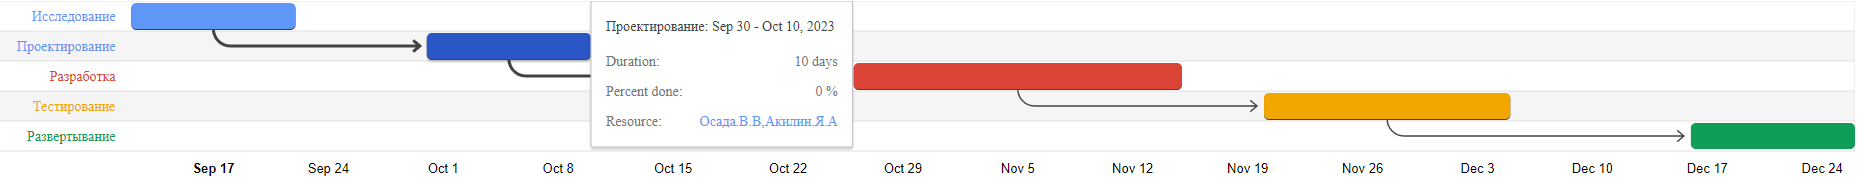
\includegraphics[width=\textwidth]{gant.png}
  \caption{Диаграмма Ганта проекта}
\end{figure}

\section{№3 Построение модели данных}

Модель данных представляет собой структуру информационной системы университета, включающую в себя сущности и связи между ними. Каждая сущность описывается набором атрибутов и может быть связана с другими сущностями с помощью отношений.

Сущности и их связи:

\begin{itemize}
  \item \textbf{Студенты}: У каждого студента есть уникальный идентификатор (ID) и личные данные (ФИО). Студенты связаны с группами по отношению "многие к одному".
  \item \textbf{Группы}: Группы имеют уникальный ID и название. Каждая группа может иметь множество студентов и связана с расписанием по отношению "одна к многим".
  \item \textbf{Преподаватели}: Преподаватели идентифицируются по ID и ФИО. Они связаны с предметами, которые преподают, по отношению "многие к многим", и с расписанием по отношению "один к многим".
  \item \textbf{Расписание}: В расписании указывается, когда и какие предметы будут преподаваться. Оно связывает преподавателей, группы и предметы.
  \item \textbf{Предметы}: Каждый предмет имеет ID, название и описание. Предметы связаны с экзаменами и расписанием по отношению "один к многим".
  \item \textbf{Экзамены}: Экзамены содержат информацию о ID, дате проведения и связанном предмете. Они связаны с предметами и группами по отношению "многие к одному".
  \item \textbf{Материалы курса}: Включают ID, название и тип материала. Они ассоциированы с предметами, по которым предоставляются, по отношению "многие к одному".
\end{itemize}

Диаграмма ниже иллюстрирует связи между сущностями:

\begin{figure}[-h]
  \centering
  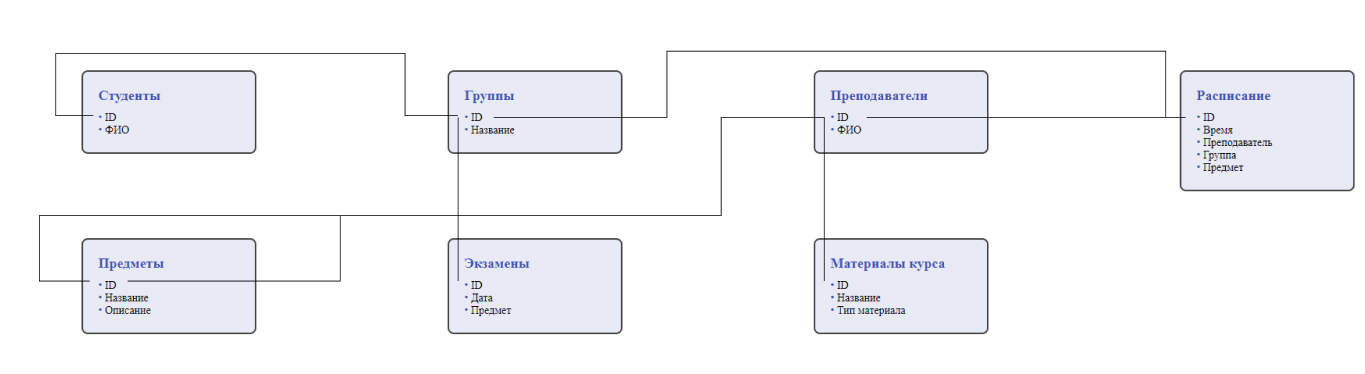
\includegraphics[width=\textwidth]{ER.png}
  \caption{ER-диаграмма информационной системы университета}
\end{figure}

\clearpage
\section*{№4 Выгрузка модели данных в СУБД и реверс инжиниринг БД}


В рамках данного этапа работы была выполнена выгрузка разработанной модели данных в систему управления базами данных (СУБД). Для демонстрации структуры базы данных и отношений между таблицами использовался процесс реверс-инжиниринга, который позволил визуализировать схему данных в виде ER-диаграммы.

Ниже представлена ER-диаграмма, отображающая связи между таблицами в базе данных:

\begin{figure}[-h]
  \centering
  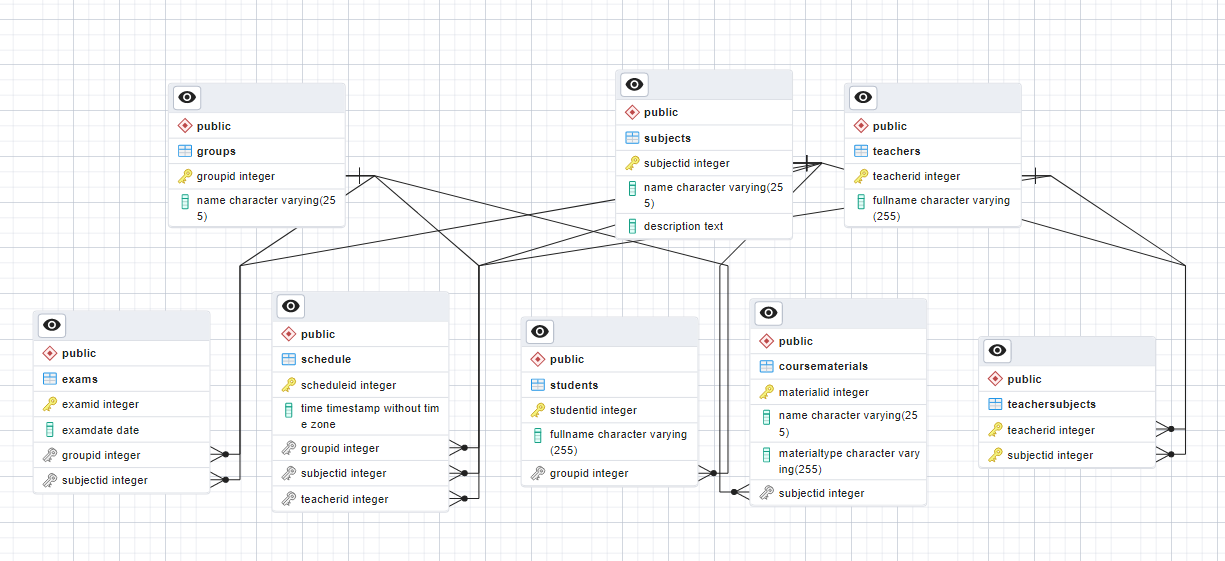
\includegraphics[width=1\linewidth]{DBER.png}
  \caption{ER-диаграмма базы данных после реверс-инжиниринга}
\end{figure}

\section*{№5 Построение функциональной модели}

\subsection{Цель работы}
Целью данной работы является разработка функциональной модели мобильного приложения университета, которая позволяет наглядно представить структуру и взаимодействие основных компонентов системы.

\subsection{Описание функциональной модели}
Представленная функциональная модель иллюстрирует основные компоненты мобильного приложения для университета и их связи. Компоненты включают:

\begin{itemize}
    \item \textbf{App}: Главный модуль, который служит входной точкой для пользователей и координирует взаимодействие между подсистемами.
    \item \textbf{User}: Основной компонент, представляющий акторов системы - студентов и преподавателей.
    \item \textbf{Students и Teachers}: Подсистемы, наследующие функции от компонента User и расширяющие их специфическими возможностями для каждой группы пользователей.
    \item \textbf{ScheduleItem}: Компонент, отвечающий за управление расписанием занятий.
    \item \textbf{Subject}: Модуль, который содержит информацию о предметах, доступных в приложении.
    \item \textbf{Exam}: Компонент, управляющий экзаменационной деятельностью в приложении.
    \item \textbf{CourseMaterial}: Раздел, в котором преподаватели могут размещать учебные материалы для студентов.
    \item \textbf{Group}: Элемент, представляющий учебные группы в системе.
\end{itemize}

\subsection{Связи между компонентами}
Каждый компонент взаимодействует с App напрямую или через другие компоненты. Пользователи (Students и Teachers) могут получать и изменять информацию о расписаниях, предметах, экзаменах и учебных материалах, в то время как компонент Group связан с ScheduleItem для предоставления информации о расписании конкретной группы.

\begin{figure}[-h]
    \centering
    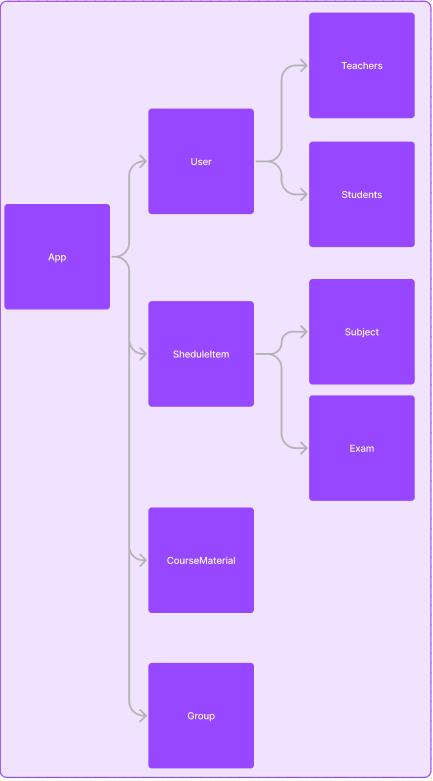
\includegraphics[width=0.5\linewidth]{func_diagram_5.png}
    \caption{Функциональная модель}
\end{figure}

\section{№6 Построение процессной модели}

\subsection{Цель работы}
Разработка процессной модели мобильного приложения для университета МАДИ, позволяющей детализировать и визуализировать потоки взаимодействия между различными видами представлений (views) в приложении.

\subsection{Описание процессной модели}
Процессная модель мобильного приложения демонстрирует потоки переходов между различными представлениями, доступными пользователям. Ключевые представления включают:

\begin{itemize}
    \item \textbf{LoginView}: Экран входа, через который пользователи получают доступ к функциям приложения после аутентификации.
    \item \textbf{RegistrationView}: Экран регистрации для создания нового пользовательского аккаунта.
    \item \textbf{ScheduleView}: Представление расписания, где пользователи могут просматривать актуальное расписание занятий.
    \item \textbf{GroupView}: Представление, которое позволяет пользователям просматривать информацию о группах и их расписаниях.
    \item \textbf{ExamView}: Экран, на котором студенты могут узнать информацию о предстоящих экзаменах.
    \item \textbf{ProfileView}: Представление профиля пользователя, где можно обновить личные данные.
    \item \textbf{MaterialView и MaterialListView}: Экраны для просмотра учебных материалов. Если пользователь является преподавателем, он может перейти к MaterialUploadView для загрузки новых материалов.
\end{itemize}

\subsection{Логика переходов}
Пользователи могут переходить между различными экранами в зависимости от своих потребностей и статуса (студент или преподаватель). Например, после успешного входа в систему через \textbf{LoginView}, студенты направляются на \textbf{ScheduleView}, а преподаватели могут перейти к загрузке материалов через \textbf{MaterialUploadView}.

\subsection{Анализ модели}
Процессная модель позволяет определить и оптимизировать потоки пользовательского опыта в приложении. Она подчеркивает удобство навигации и доступность функций приложения для различных пользовательских ролей.

\begin{figure}[-h]
    \centering
    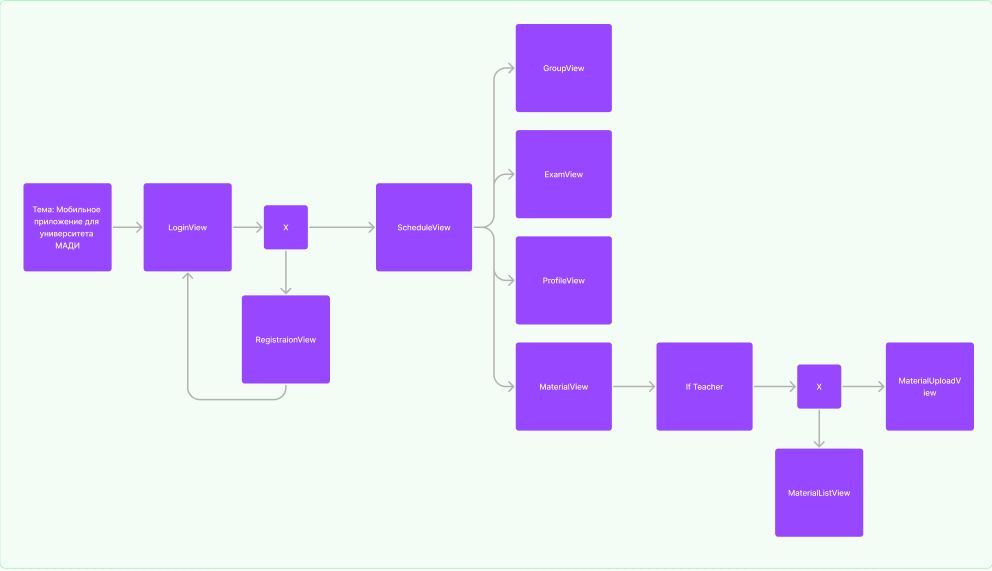
\includegraphics[width=1\linewidth]{processModel.png}
    \caption{Процессная модель}
    
\end{figure}

\section{№7 Построение модели потоков данных}

\subsection{Цель работы}
Разработка модели потоков данных для мобильного приложения университета МАДИ, позволяющей визуализировать и анализировать передачу информации между различными акторами и системами.

\subsection{Описание модели потоков данных}
Модель потоков данных показывает взаимодействие между участниками образовательного процесса и информационной системой. Включает в себя следующие элементы:

\begin{itemize}
    \item \textbf{Teacher}: Преподаватель загружает учебные материалы и взаимодействует с базой данных для управления курсами и оценками студентов.
    \item \textbf{Student}: Студент имеет доступ к расписанию, учебным материалам и своему профилю через мобильное приложение.
    \item \textbf{PostgreSQL}: Центральная база данных, которая хранит всю информацию, связанную с учебным процессом, включая учебные материалы, расписание и профили пользователей.
    \item \textbf{DevOps}: Инструменты и процессы, используемые для непрерывной интеграции и развертывания приложения, что обеспечивает актуальность данных и доступность сервиса.
\end{itemize}

\subsection{Потоки данных}
Потоки данных включают запросы и обновления, производимые преподавателями и студентами:

\begin{itemize}
    \item \textbf{Material Upload}: Преподаватели загружают материалы, которые затем хранятся в базе данных PostgreSQL.
    \item \textbf{Request}: Студенты отправляют запросы на получение данных, таких как расписание и учебные материалы, из базы данных.
\end{itemize}

\begin{figure}
    \centering
    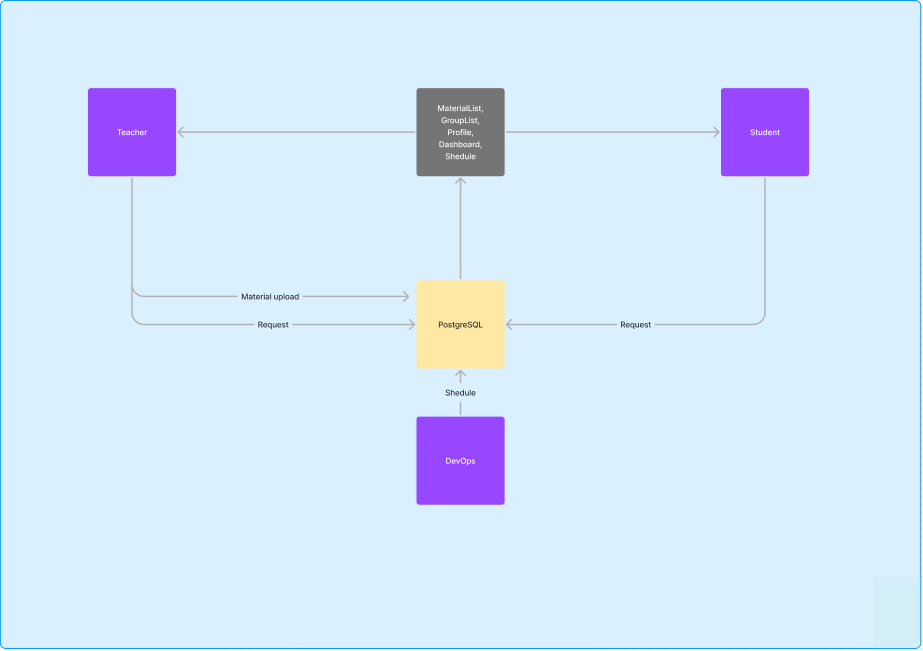
\includegraphics[width=1\linewidth]{Arch_program_compl.png}
    \caption{Модель потоков данных}
\end{figure}

\clearpage
\section*{№9 UML. Диаграмма классов}

\subsection{Цель работы}
Применение диаграммы классов для описания структуры выбранного решения и ознакомление с инструментами, позволяющими строить диаграмму классов.

\subsection{Задание}
В соответствии с заданием лабораторной работы №3 разработать диаграмму классов для описания структуры выбранного решения. Диаграмма классов должна чётко отражать все основные компоненты системы, их атрибуты, методы и взаимосвязи.

\subsection{Методология}
Для разработки диаграммы классов были использованы следующие принципы объектно-ориентированного проектирования:
\begin{itemize}
    \item Инкапсуляция данных и поведения в классах.
    \item Абстракция для определения ключевых характеристик классов.
    \item Наследование для создания иерархии классов и переиспользования кода.
    \item Полиморфизм для использования объектов производных классов через интерфейс базового класса.
\end{itemize}

\subsection{Результаты}
В результате были идентифицированы и описаны ключевые классы системы, включая \textit{User}, \textit{Student}, \textit{Teacher}, и другие. Были определены основные атрибуты и методы каждого класса, а также отношения между классами, такие как ассоциации, зависимости и наследование.

\begin{figure}[-h]
    \centering
    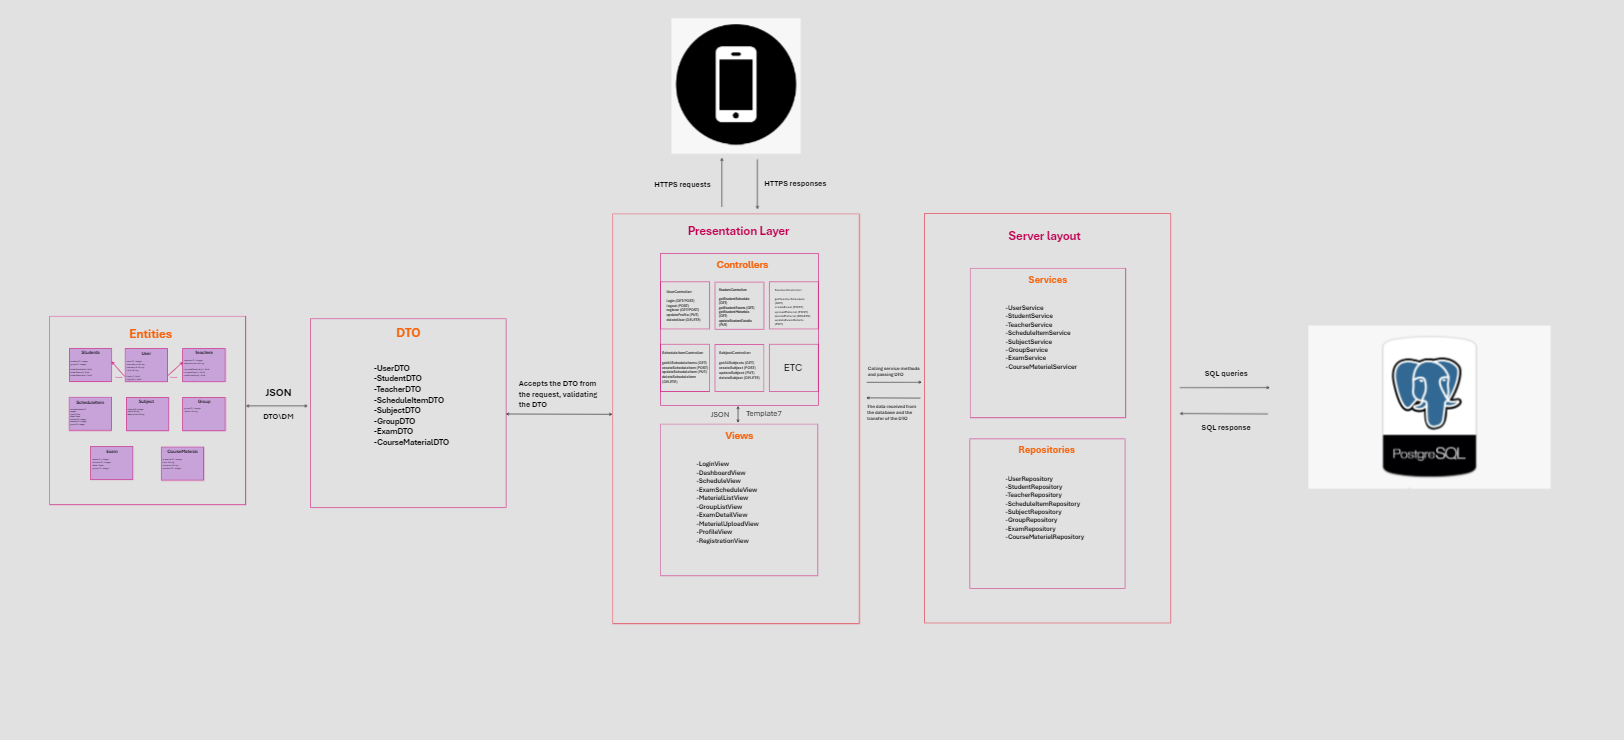
\includegraphics[width=0.5\linewidth]{UML_Class.png}
    \caption{UML диаграмма классов}
\end{figure}

\section{№10 UML. Диаграммы объектов}

\subsection{Цель работы}
Целью данной работы является применение диаграммы объектов UML для наглядного представления структуры выбранного программного решения, показывающей объекты системы, их атрибуты и взаимосвязи в определённый момент времени.

\subsection{Задание}
На основе результатов лабораторной работы №9 по созданию диаграммы классов разработать диаграмму объектов, которая детализирует взаимодействие между экземплярами классов в рамках выбранной системы. Диаграмма объектов должна включать экземпляры таких классов, как \textit{User}, \textit{Student}, \textit{Teacher}, \textit{ScheduleItem}, \textit{Subject}, \textit{Group}, \textit{Exam} и \textit{CourseMaterial}.

\subsection{Методика выполнения}
Для каждого класса были созданы уникальные объекты с их атрибутами и отношениями. В качестве примера, объект класса \textit{Student} может быть представлен следующим образом:
\begin{itemize}
    \item student1: \textit{Student}
    \begin{itemize}
        \item studentID: 1001
        \item groupID: 501
        \item username: "OsadaV"
        \item password: "jd\_secure123"
        \item role: "student"
        \item \ldots
    \end{itemize}
\end{itemize}
Аналогичные объекты созданы для других классов, отражая их реальные экземпляры в рамках системы.

\subsection{Результаты}
Была разработана диаграмма объектов, позволяющая визуализировать статическую структуру системы на примере конкретных объектов. Она демонстрирует, как объекты могут быть созданы, какие данные они хранят и как между ними происходит взаимодействие.

\begin{figure}[-h]
    \centering
    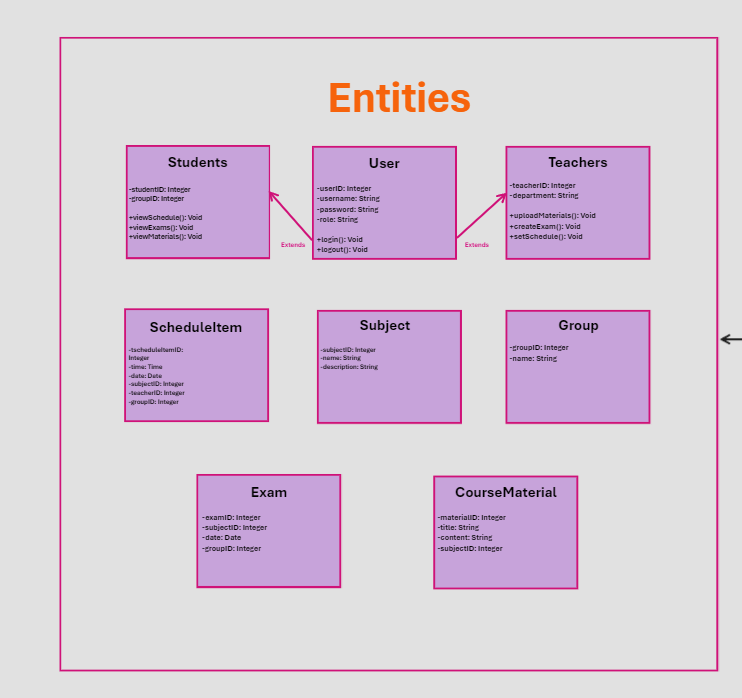
\includegraphics[width=0.5\linewidth]{UML_Obj.png}
    \caption{UML диаграмма обьектов}
\end{figure}

\section{№11 UML. Диаграмма вариантов использования}

\subsection{Цель работы}
Целью данной работы является использование диаграммы вариантов использования для наглядного представления функциональных требований к разрабатываемой системе, а также ознакомление с инструментарием для создания UML диаграмм.

\subsection{Описание диаграммы вариантов использования}
Диаграмма вариантов использования для системы мобильного приложения университета позволяет наглядно представить ключевые функции, доступные двум основным актерам системы: студентам и преподавателям.

\begin{itemize}
    \item \textbf{Студент} может выполнять следующие операции:
    \begin{itemize}
        \item Регистрация/вход в систему
        \item Обновление профиля
        \item Общение в чате
        \item Просмотр оценок
        \item Просмотр расписаний
        \item Просмотр учебных материалов
        \item Просмотр экзаменов
    \end{itemize}
    \item \textbf{Преподаватель} имеет возможность:
    \begin{itemize}
        \item Регистрация/вход в систему
        \item Обновление профиля
        \item Общение в чате
        \item Создание экзаменов
        \item Загрузка учебных материалов
        \item Оценка студентов
        \item Управление расписанием занятий
    \end{itemize}
\end{itemize}

\subsection{Сценарии использования}
\subsubsection{Регистрация/вход в систему}
Основной поток событий для сценария регистрации/входа в систему начинается, когда студент или преподаватель выбирает опцию регистрации или входа в приложении. Пользователь вводит необходимые данные, и система обрабатывает их для аутентификации или регистрации нового профиля.

\subsubsection{Просмотр расписаний}
Студент выбирает опцию просмотра расписаний. Приложение отображает актуальное расписание занятий. В случае отсутствия интернет-соединения пользователю предлагается последнее сохранённое офлайн расписание.

\subsubsection{Создание экзаменов}
Преподаватель выбирает опцию создания экзамена, вводит необходимые данные и публикует экзамен для группы студентов.

\begin{figure}[-h]
    \centering
    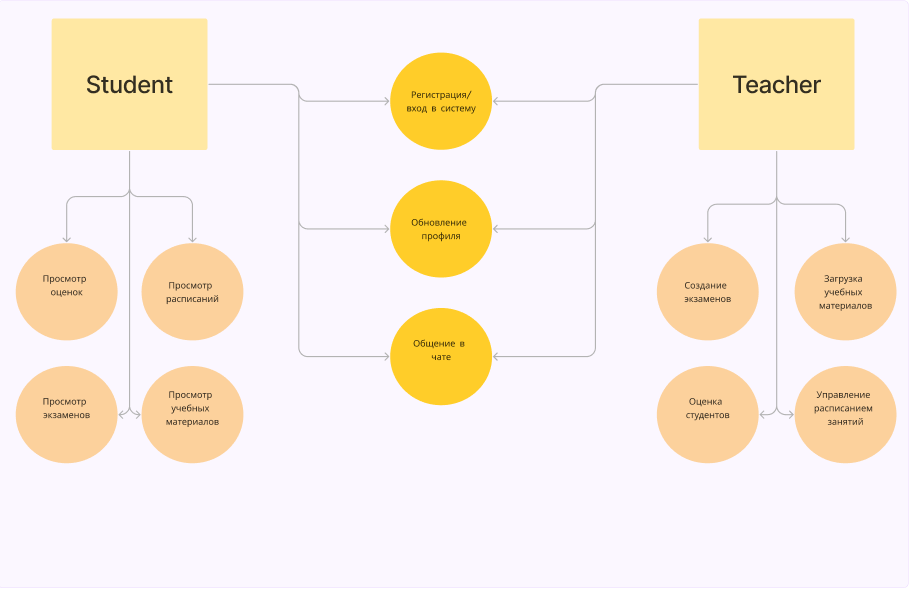
\includegraphics[width=1\linewidth]{UML_variation_use.png}
    \caption{UML.Диаграмма вариантов использования}
\end{figure}

\section{№12 UML. Диаграмма последовательности}

\subsection{Цель работы}
Применение диаграммы последовательности для детального описания процессов внутри разрабатываемой системы, позволяющее визуализировать порядок взаимодействия между объектами системы.

\subsection{Описание диаграммы последовательности}
На диаграмме последовательности представлен процесс регистрации пользователя в системе. Диаграмма включает в себя следующие шаги:

\begin{enumerate}
    \item Пользователь вводит свои данные на форме регистрации и нажимает кнопку "Зарегистрироваться".
    \item UI отправляет запрос на \texttt{RegistrationController}.
    \item \texttt{RegistrationController} принимает данные и обращается к \texttt{RegistrationService}.
    \item \texttt{RegistrationService} запрашивает у \texttt{UserRepository} добавление нового пользователя.
    \item \texttt{UserRepository} выполняет запрос к базе данных для сохранения информации.
    \item База данных подтверждает сохранение и возвращает подтверждение обратно к \texttt{UserRepository}.
    \item \texttt{UserRepository} возвращает результат в \texttt{RegistrationService}.
    \item \texttt{RegistrationService} передает результат в \texttt{RegistrationController}.
    \item \texttt{RegistrationController} отправляет ответ об успешной регистрации на UI.
    \item UI отображает пользователю сообщение об успешной регистрации.
\end{enumerate}

\subsection{Анализ диаграммы}
Диаграмма последовательности демонстрирует взаимодействие между пользовательским интерфейсом, контроллером, сервисом и репозиторием, а также их связь с базой данных. Это позволяет отследить жизненный цикл запроса пользователя от начала до конца и является основой для понимания и разработки бэкенд-логики системы.

\begin{figure}[-h]
    \centering
    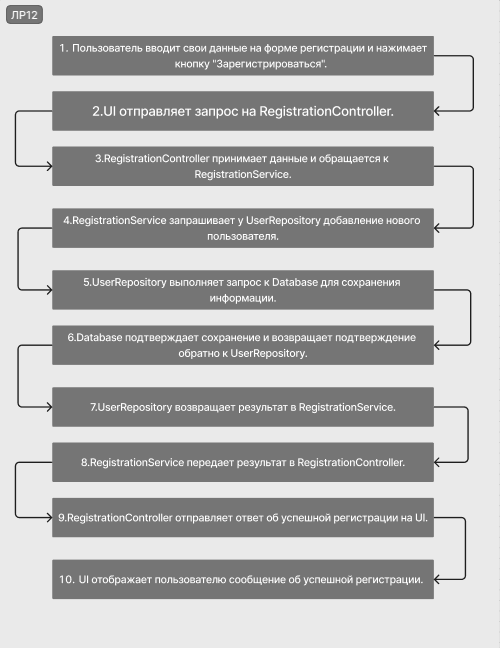
\includegraphics[width=0.5\linewidth]{UML_serial.png}
    \caption{UML. Диаграмма последовательности}
\end{figure}

\clearpage
\section{№13UML. Диаграмма сотрудничества}

\subsection{Цель работы}
Применение диаграммы сотрудничества для визуализации взаимодействий между различными компонентами системы при процессе регистрации пользователя.

\subsection{Описание диаграммы}
Диаграмма сотрудничества показывает процесс регистрации пользователя, включая следующие компоненты системы:

\begin{itemize}
    \item \textbf{Пользовательский интерфейс}: Место, где пользователь вводит свои данные для регистрации.
    \item \textbf{Контроллер регистрации}: Получает данные от пользователя и отправляет запрос на регистрацию в сервис регистрации.
    \item \textbf{Сервис регистрации}: Обрабатывает запрос на регистрацию и взаимодействует с репозиторием пользователей.
    \item \textbf{База данных}: Хранит информацию о пользователях и обрабатывает запросы на сохранение новых данных.
    \item \textbf{Репозиторий пользователей}: Служит посредником между сервисом регистрации и базой данных.
\end{itemize}

Каждый компонент связан со следующим через определенные действия, такие как \textit{Регистрация/Данные}, \textit{Запрос на регистрацию}, \textit{Подтверждение на сохранение данных/ошибка}, и \textit{Взаимодействие данными}.

\subsection{Взаимодействия}
\begin{enumerate}
    \item Пользователь вводит данные в пользовательском интерфейсе и инициирует процесс регистрации.
    \item Контроллер регистрации принимает данные и отправляет их в сервис регистрации.
    \item Сервис регистрации обрабатывает данные и делегирует задачу сохранения информации репозиторию пользователей.
    \item Репозиторий пользователей взаимодействует с базой данных для сохранения информации.
    \item База данных возвращает результат операции репозиторию пользователей, который, в свою очередь, информирует сервис регистрации.
    \item Сервис регистрации отправляет результат контроллеру регистрации.
    \item Контроллер регистрации возвращает результат операции в пользовательский интерфейс.
    \item Пользовательский интерфейс отображает сообщение об успешной регистрации или об ошибке.
\end{enumerate}

\begin{figure}[-h]
    \centering
    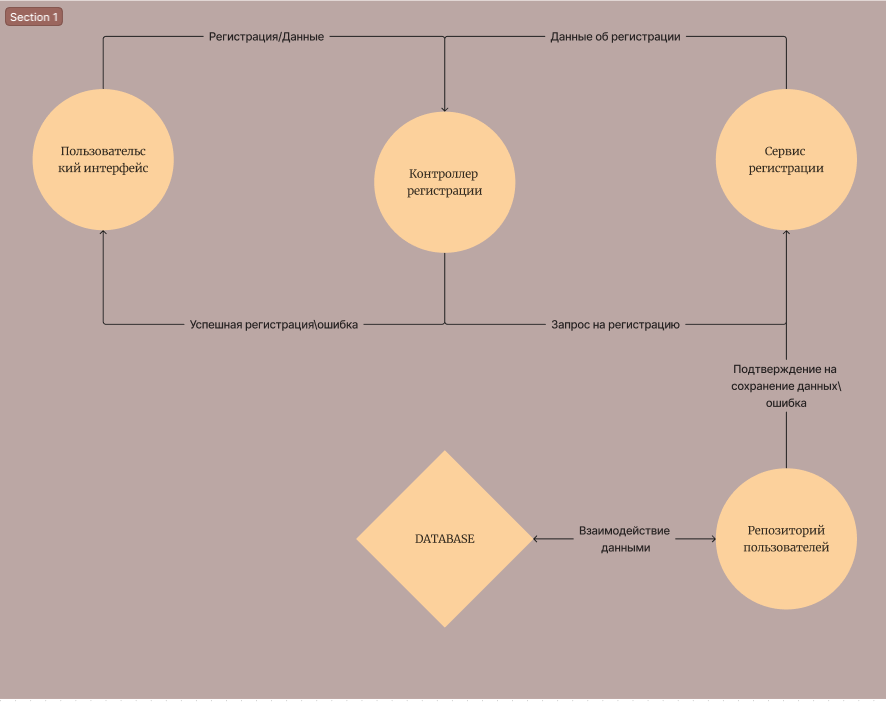
\includegraphics[width=1\linewidth]{UML_Sotr.png}
    \caption{UML. Диаграмма сотрудничества}
\end{figure}

\section{№14 UML. Диаграмма схем состояний}

\subsection{Цель работы}
Цель данной работы — создание UML диаграммы схемы состояний, отображающей жизненный цикл пользователя в системе мобильного приложения университета МАДИ.

\subsection{Описание диаграммы схемы состояний}
Диаграмма схемы состояний визуализирует различные состояния, через которые проходит пользователь во время взаимодействия с системой. На диаграмме отображены следующие состояния:

\begin{itemize}
    \item Начальное состояние, где пользователь начинает взаимодействие с системой.
    \item Процесс аутентификации, который определяет, является ли пользователь авторизованным или нет.
    \item Авторизованный пользователь получает доступ к функциям системы, таким как просмотр расписания и учебных материалов.
    \item Не авторизованный пользователь направляется к процессу аутентификации или к просмотру общедоступной информации.
    \item Для администраторов и сотрудников БД предусмотрены дополнительные функции, связанные с управлением системой.
\end{itemize}

\subsection{Переходы между состояниями}
Переходы между состояниями осуществляются посредством событий, таких как успешная аутентификация или запрос на просмотр данных. Каждый переход четко определен и управляется системой безопасности.

\begin{figure}[-h]
    \centering
    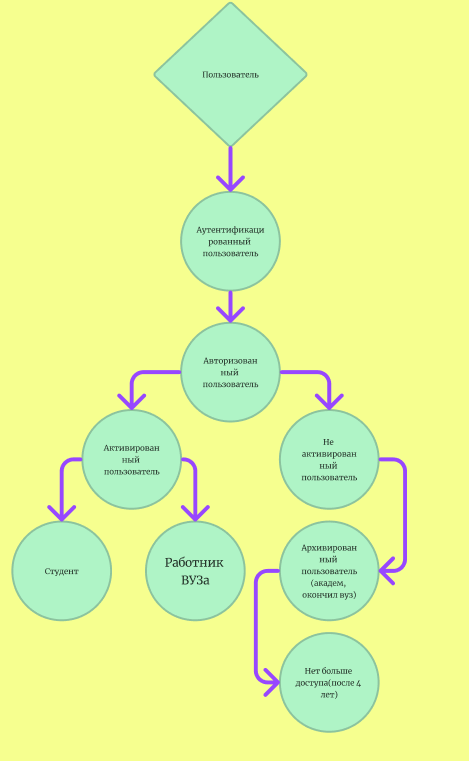
\includegraphics[width=0.5\linewidth]{14UML.png}
    \caption{Диаграмма состояний}
\end{figure}

\clearpage
\section{№15 UML. Диаграмма деятельности}

\subsection{Цель работы}
Целью данной работы является использование UML диаграммы деятельности для описания различных потоков взаимодействия акторов с мобильным приложением университета МАДИ.

\subsection{Описание диаграммы}
Диаграмма деятельности представляет потоки действий, которые выполняются различными акторами системы. Включает в себя следующие процессы и акторы:

\begin{itemize}
    \item \textbf{Студенты}, выполняющие действия такие как просмотр расписания и материалов, а также сдача заданий.
    \item \textbf{Преподаватели}, занимающиеся загрузкой материалов и оценкой студентов.
    \item \textbf{Административный персонал}, управляющий профилем и вносящий изменения в расписание, а также добавляющий новые функционалы в систему.
\end{itemize}


\begin{figure}[-h]
    \centering
    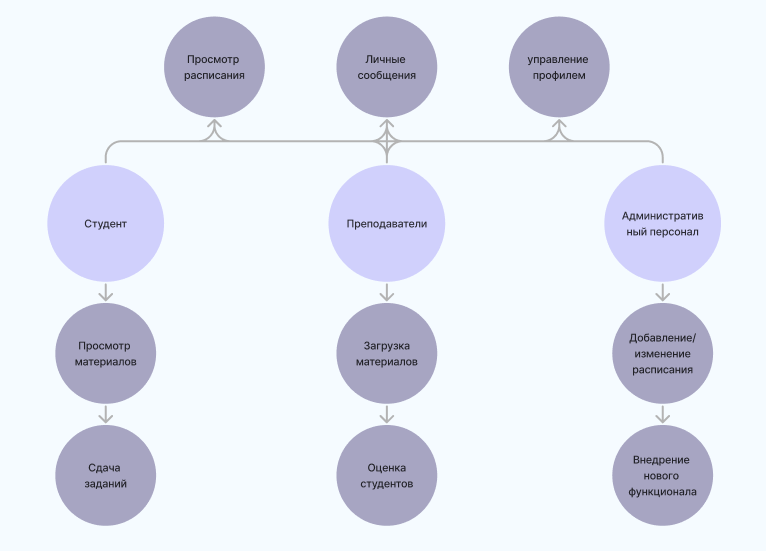
\includegraphics[width=0.5\linewidth]{15UML.png}
    \caption{Диаграмма состояний}
\end{figure}

\section{№16 UML. Компонентная диаграмма}

\subsection{Цель работы}
Целью работы является разработка компонентной диаграммы для мобильного приложения университета МАДИ, отображающей структуру и взаимосвязь между различными модулями и их интерфейсами.

\subsection{Описание компонентов}
На диаграмме представлены следующие основные компоненты системы:
\begin{itemize}
  \item Пользователи, разделенные на преподавателей и студентов.
  \item Специализированные компоненты для каждой группы пользователей, обеспечивающие доступ к соответствующим данным, таким как лекции, бакалавриаты, специальности, аспирантуры и т.д.
  \item Компоненты данных, такие как расписание, литература, распределение и предметы, которые управляют соответствующей информацией в системе.
  \item Материалы, связанные с учебным процессом и доступные для пользователей.
\end{itemize}

\subsection{Взаимодействие между компонентами}
Каждый компонент системы обеспечивает определенный интерфейс, через который он взаимодействует с другими компонентами:
\begin{itemize}
  \item Преподаватели и студенты взаимодействуют с системой через предоставленные им компоненты, которые позволяют обращаться к требуемым данным.
  \item Компоненты данных предоставляют интерфейсы JSON для интеграции с сервером приложений и обработки запросов от пользователей.
\end{itemize}


\begin{figure}[-h]
    \centering
    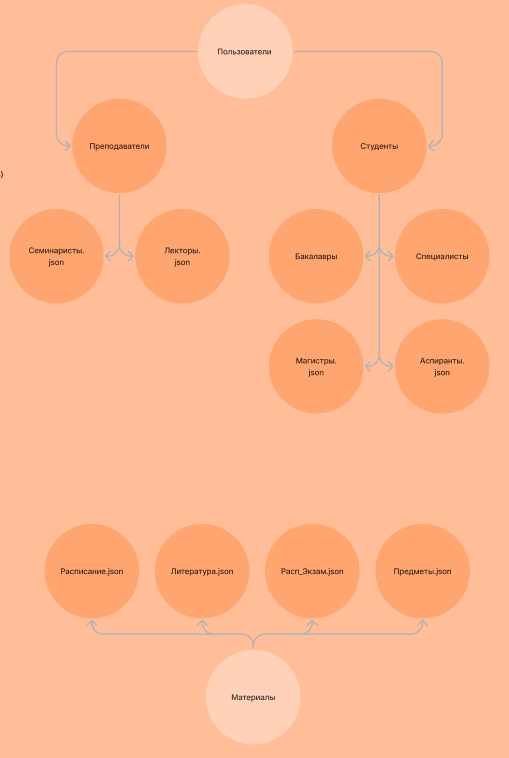
\includegraphics[width=0.5\linewidth]{16UML.png}
    \caption{Диаграмма состояний}
\end{figure}


\section{№17 UML. Диаграмма размещения}

\subsection{Цель работы}
Целью данной работы является разработка UML диаграммы размещения для иллюстрации физического развертывания компонентов системы мобильного приложения университета МАДИ в рамках аппаратной инфраструктуры.

\subsection{Описание диаграммы}
На представленной диаграмме размещения иллюстрируются следующие компоненты системы:
\begin{itemize}
  \item \textbf{Пользователи} — отображают физические точки входа в систему, через которые осуществляется доступ к мобильному приложению.
  \item \textbf{Сервер} — центральный узел системы, который обрабатывает входящие запросы от пользователей и взаимодействует с базой данных.
  \item \textbf{База данных} — хранит все данные, необходимые для функционирования мобильного приложения.
\end{itemize}

\subsection{Физическое развертывание}
Каждый из пользователей подключается к серверу, который в свою очередь связан с базой данных. Это развертывание позволяет пользователям взаимодействовать с централизованным хранилищем данных через сервер приложений.

\subsection{Взаимодействие компонентов}
Пользователи отправляют запросы на сервер, который обрабатывает эти запросы и, при необходимости, обращается к базе данных для извлечения или сохранения информации. Затем сервер отправляет ответы обратно пользователям. Вся коммуникация между пользователями и сервером, а также между сервером и базой данных осуществляется через защищенные соединения.

\begin{figure}[-h]
    \centering
    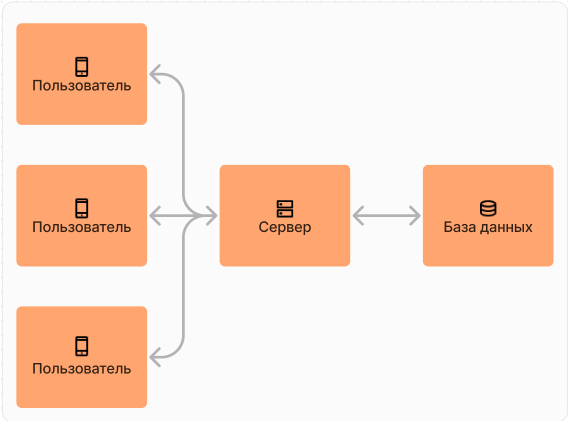
\includegraphics[width=0.5\linewidth]{17UML.png}
    \caption{Диаграмма состояний}
\end{figure}

\end{document}
